\documentclass{article}
\usepackage[utf8]{inputenc}
\usepackage{graphicx}
\usepackage{hyperref}
\usepackage{float}
\usepackage[export]{adjustbox}

\title{Proof Of Concept Design}
\author{Sophie Wallace }
\date{September 2019}

\begin{document}

\maketitle
\tableofcontents
\clearpage

\section{Introduction}
This Proof of Concept (PoC) design draws from extensive scoping and testing conducted in tasks Scoping II, Elaboration I and II. These tasks sought to identify appropriate tools and techniques necessary to solve the pains that are frequently experienced in anthropological fieldwork. Through these tests, I established the most significant gain creator would be a technology that assists with organising and storing data from the field including notes, images, audio and video. Additional features of this tool will be discussed further in the user stories.  


\section{User Stories}
A user story is a method to add business value by capturing requirements from user perspective in the form of some description (SYSTANGO 2019). User stories are vital in understanding the features that users value and prioritise. For this PoC, user stories will address the required features for this PoC to be eventually demonstrated. \textbf{Figure 1} displays the concept of the 3 Rs needed for a contextual and concise user story (SYSTANGO 2019).

\begin{figure}[H]
    \centering
    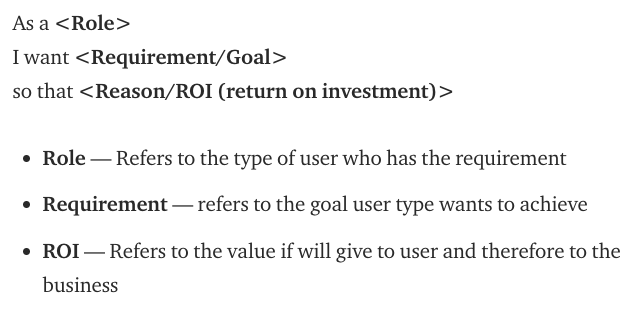
\includegraphics[width=\textwidth, frame]{UserStories_ThreeRs.png}
    \caption{3 Rs of User Stories}
    \label{fig:my_label}
\end{figure} 

For each of the user stories provided below, acceptance criteria will then follow. This aims to articulate exactly when the user story is done from product owners perspective to produce acceptance tests (SYSTANGO 2019). As this technology is targeted to assist with ethnographic data management, each user story will be from the perspective of an anthropologist.
\clearpage



    

\begin{itemize}
\item As an anthropologist, I want the data collected on my mobile to be transferred to my laptop so I can have a streamlined process for data collection and storage.
\item As an anthropologist, I want all of my ethnographic data types such as text, photos, video and audio, to be organised in one space. This will help manage large data sets and save time finding or categorising data collected in the field. 
\item As an anthropologist, I want all my collected data to have rich metadata so I can conveniently identify the defining features of each data type.
\item As an anthropologist, I want to be able to edit data types so I can add, adjust and refine collected data.
\item As an anthropologist, I want my technology to function offline so I can avoid depending on internet connection.
\item As an anthropologist, I want to be able to store collected data in an external system so I can ensure all materials are secure and backed up.  
\end{itemize}






\section{Acceptance Criteria}

\section{Themes in User Stories}

\section{References}
SYSTANGO. 2019. “working ” Medium. Medium. January 11, 2019. \.Perkel, Jeffrey M. 2019. “Workflow Systems Turn Raw Data into Scientific Knowledge.” Nature 573 (7772): 149–50. https://doi.org/10.1038/d41586-019-02619-z

\end{document}
